\chapter{Fixed Income}
\begin{fquote}[John von Neumann][1903-1957]If people do not believe that mathematics is simple, it is only because they do not realize how complicated life is.
\end{fquote}

\section{Compounding}

\subsection{Discrete}
\subsubsection{Linear}

$FV$, the future value in $T$ periods of a nominal $N$, is expressed as:

\[
FV_T = N(1+R_TT)
\]

where $R_T$ is the interest rate.

\subsubsection{Exponential}

Future value of a nominal cash flow $N$ under exponential compounding over
$n$ periods:

\[ FV_T = N(1+R_T)^n \]

The present value of a nominal future cash flow $N$ is therefore:

\[ PV_T = \frac{N}{(1+R_T)^n} \]

Periodic compounding where $n$ is the number of times interest compounded per period

\[ 
FV_T=N\left( 1 + \frac{R}{n}  \right)^{nT}
\]

\subsection{Continuous}
Continuous compounding is defined as taking the limit of the periodic compounding as n goes to infinity,
\[ 
FV=\lim_{n \to \infty} N \left(1+\frac{R}{n}\right)^{nT}=Ne^{RT}
\]

\subsection{Transition between discrete and continuous}
Table of interest rates at various compounding frequencies.

%\ab{Jost said we need to describe the table here}

\ctable[
caption = Interest rates at various compounding frequencies,
pos = ht,
doinside=\small
]{lllllll}{
}{
\toprule
 Nominal Rate &  Semi-Annual & Quarterly &  Monthly &  Weekly &  Daily  & Continuous \\
  \midrule
    1.0000       & 1.0025       & 1.0038     & 1.0046   & 1.0049  & 1.0050  & 1.0050      \\
    2.0000       & 2.0100       & 2.0151     & 2.0184   & 2.0197  & 2.0201  & 2.0201      \\
    5.0000       & 5.0625       & 5.0945     & 5.1162   & 5.1246  & 5.1267  & 5.1271      \\
    10.0000      & 10.2500      & 10.3813    & 10.4713  & 10.5065 & 10.5156 & 10.5171     \\
    15.0000      & 15.5625      & 15.8650    & 16.0755  & 16.1583 & 16.1798 & 16.1834     \\
    20.0000      & 21.0000      & 21.5506    & 21.9391  & 22.0934 & 22.1336 & 22.1403     \\
    25.0000      & 26.5625      & 27.4429    & 28.0732  & 28.3256 & 28.3916 & 28.4025     \\
    50.0000      & 56.2500      & 60.1807    & 63.2094  & 64.4788 & 64.8157 & 64.8721     \\ 
  \bottomrule
}

\section{Interest rates}
\ctable[
caption = The caption is centered by default,
pos = h,
doinside=\small,
center,
]{llll}{
}{
\toprule
    Maturity (months) & Spot rate & Forward & Rate \\
  \midrule
    3 & 4.5\% & $F_{0,3}$ & 4.5\% \\
    6 & 4.3\% & $F_{3,3}$ & 4.05\% \\
    9 & 4.2\% & $F_{6,3}$ & 3.92\% \\
    12 & 4.0\% & $F_{9,3}$ & 3.3\% \\
  \bottomrule
}

\subsection{Spot rates}

\subsection{Forward rates}
Forward rates indicate the interest rate between two future dates [S,T]
\[
(1+R_T)^T=(1+R_S)^S(1+R(t;S,T))^{T-S}; T>S
\]
Solving for the forward rate yields
\[
R(t=0,S,T)=\left( \frac{(1+R_T)^T}{(1+R_S)^S} - 1 \right)^{\frac{1}{T-S}};T>S
\]

Continuous compounding version of the above

\[
e^{R_TT}=e^{R_SS}e^{R(t;S,T)(T-S)};T>S
\]
Solving for the forward rate
\[
R(t;S,T)=\frac{R_TT-R_SS}{T-S}
\]

\subsection{LIBOR}
The LIBOR (London InterBank Offered Rate) interest rate is the most important interbank rate
used for fixed income valuation. LIBOR rates are quoted on a simple compounding basis with maturities
from overnight to 12 months.
\\
\\
Table of LIBOR rates per 2013-12-26,

\ctable[
caption = LIBOR rates 2013-12-26,
pos = ht,
width=60mm,
center,
doinside=\small
]{ll}{
}{
  \toprule
    Period & LIBOR \\
  \midrule
    1 month & 0.17\% \\ 
    3 month & 0.24\% \\
    6 month & 0.35\% \\
    12 month & 0.59\% \\
  \bottomrule
}


%$R$ is the annual rate
%The value after m compounding periods with n compounding periods per year

\[ 
1+(T-S)L=\frac{p(t,S)}{p(t,T)}
\]
\[ 
e^{r(T-S)}=\frac{p(t,S)}{p(t,T)}
\]
\\
\textbf{LIBOR forward rate}
Simply-compounded forward rate $[S,T]$ prevailing at time $t$,
\[
L(S,T) = -\frac{p(S,T)-p(t,S)}{(T-S)p(t,T)}
\]
\\
\textbf{LIBOR spot rate},

\[
L(S,T)=\frac{p(S,T)-1}{(T-S)p(S,T)}
\]
\\
\textbf{LIBOR forward rate},
Continuously compounded forward rate $[S,T]$ prevailing at time $t$,

\[
R(t;S,T)=-\frac{\log{p(t,T)}-\log{p(t,S)}}{T-S}
\]
\\
\textbf{LIBOR spot rate},
\[
R(S,T)=\frac{\log{p(S,T)}}{T-S}
\]
\\
\textbf{Instantaneous forward rate},
\[
f(t,T)=-\frac{\partial\log{p(t,T)}}{\partial{T}}
\]
\\
\textbf{Instantaneous short rate},
\[
r(t)=f(t,t)
\]

For example, the three-month forward LIBOR for the period $[S,T]$, where $T=S+\tau$ and $\tau=1/4$,
\[
L(t,T) = F(t;S,S+\tau) = F(t;S,T), T>S
\]

\subsubsection{Calculating LIBOR rates}

\section{Bonds}

\subsection{Zero coupon bond}
Zero coupon bond and the discount factor

\subsection{Fixed coupon bond}
Series of payments called coupons and a nominal value N (face value)
A number of future payment dates $T_1 < ... < T_n$ where is the maturity of the bond
A sequence of deterministic coupons $c_1, ..., c_n$

\[ c_{T_i} = \left\{
\begin{array}{ll}
  Nc, & \text{for } i=1,...,n-1,  \\
  N(c+1), &\text{for } i=n.
\end{array} \right.\]

\[
p(t) = N \cdot p(t,T_n)+\sum_{i=1}^{n} (c_ip(t,T_i))
\]
From above, we can see that the fixed coupon bond can be reconstructed by a portfolio of zero
bonds (scaled by the coupon), $p(t,T)$ is a zero bond with N=1.
\[
p(t)=\left[p(t,T_n)+r\delta\sum_{i=1}^{n} p(t,T_i)\right]\cdot N
\]
Where $r$ is the coupon rate. For a standardized coupon bond the time intervals will be equally
spaced according to
\[
T_i=T_0+i\delta
\]

Convert above to a list of payments at offset times. Where denotes the time interval in years
according to the day-count convention, see below.

\subsection{Annuity}

An annuity is an example of an amortized bond meaning that the debitor repays the
face value over its lifetime. Payments are distributed equally over all the settlement
dates, increasing and decreasing the repayment amount and coupon respectively (see figure
\ref{fig:annuitycf}.

\begin{figure}[h!]
\begin{center}
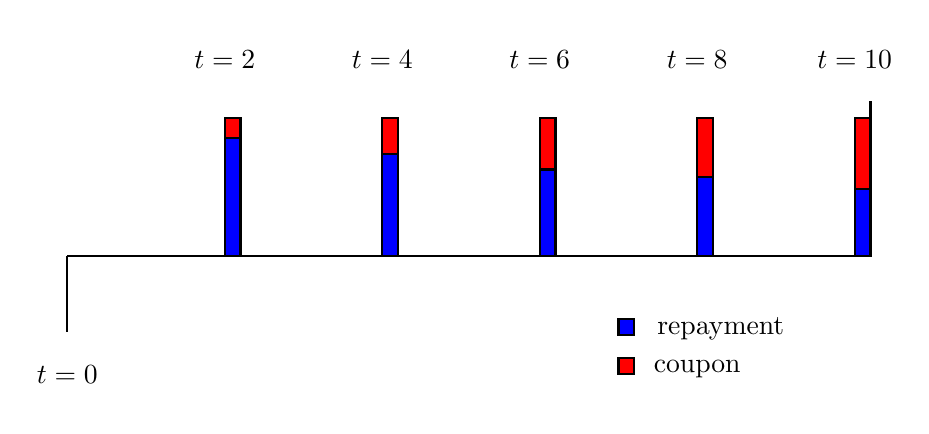
\begin{tikzpicture}[-,shorten >=1pt,auto,node distance=1.5cm,thick,minimum size=0.8cm,main node/.style={circle,draw=red,very thick}]
\tikzstyle{selected edge} = [draw,line width=6pt,-,blue!30]

\coordinate (belowstart) at (0,-1);
\coordinate (start) at (0,0);
\coordinate (stop) at (10.2,0);
\coordinate (abovestop) at (10.2,2);
\draw (start) -- (stop);
\draw (start) -- (belowstart);
\draw (stop) -- (abovestop);

\node at (0, -1.5) () {$t=0$};

\filldraw[draw=black, fill=blue] (2,0) rectangle node {} +(0.2,1.5);
\filldraw[draw=black, fill=red]  (2,1.5) rectangle node {} +(0.2,0.25);
\node at (2, 2.5) () {$t=2$};

\filldraw[draw=black, fill=blue] (4,0) rectangle node {} +(0.2,1.3);
\filldraw[draw=black, fill=red]  (4,1.3) rectangle node {} +(0.2,0.45);
\node at (4, 2.5) () {$t=4$};

\filldraw[draw=black, fill=blue] (6,0) rectangle node {} +(0.2,1.1);
\filldraw[draw=black, fill=red]  (6,1.1) rectangle node {} +(0.2,0.65);
\node at (6, 2.5) () {$t=6$};

\filldraw[draw=black, fill=blue] (8,0) rectangle node {} +(0.2,1);
\filldraw[draw=black, fill=red]  (8,1) rectangle node {} +(0.2,0.75);
\node at (8, 2.5) () {$t=8$};

\filldraw[draw=black, fill=blue] (10,0) rectangle node {} +(0.2,0.85);
\filldraw[draw=black, fill=red]  (10,0.85) rectangle node {} +(0.2,0.9);
\node at (10, 2.5) () {$t=10$};

% Legend
\filldraw[draw=black, fill=blue] (7,-1) rectangle node {} +(0.2,0.2);
\node at (8.3, -0.92) () {repayment};

\filldraw[draw=black, fill=red] (7,-1.5) rectangle node {} +(0.2,0.2);
\node at (8, -1.44) () {coupon};

\end{tikzpicture}
\caption{Cashflow of an annuity.}
\label{fig:annuitycf}
\end{center}
\end{figure}



\subsection{Bullet}

Bullet has a fixed rate coupon which is paid at every settlement. No repayments before maturity. Figure \ref{fig:bulletcf} shows the cashflows.

\[ p(t,T) = \sum_{t=1}^{T}\frac{C}{(1+r)^t} + \frac{N}{(1+r)^T} \]

\begin{figure}[h!]
\begin{center}
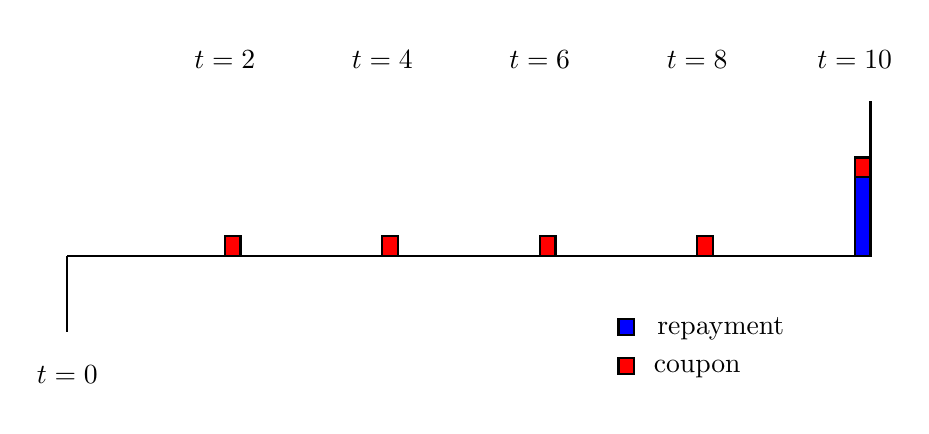
\begin{tikzpicture}[-,shorten >=1pt,auto,node distance=1.5cm,thick,minimum size=0.8cm,main node/.style={circle,draw=red,very thick}]
\tikzstyle{selected edge} = [draw,line width=6pt,-,blue!30]

\coordinate (belowstart) at (0,-1);
\coordinate (start) at (0,0);
\coordinate (stop) at (10.2,0);
\coordinate (abovestop) at (10.2,2);
\draw (start) -- (stop);
\draw (start) -- (belowstart);
\draw (stop) -- (abovestop);

\node at (0, -1.5) () {$t=0$};

\filldraw[draw=black, fill=red]  (2,0) rectangle node {} +(0.2,0.25);
\node at (2, 2.5) () {$t=2$};

\filldraw[draw=black, fill=red]  (4,0) rectangle node {} +(0.2,0.25);
\node at (4, 2.5) () {$t=4$};

\filldraw[draw=black, fill=red]  (6,0) rectangle node {} +(0.2,0.25);
\node at (6, 2.5) () {$t=6$};

\filldraw[draw=black, fill=red]  (8,0) rectangle node {} +(0.2,0.25);
\node at (8, 2.5) () {$t=8$};

\filldraw[draw=black, fill=blue] (10,0) rectangle node {} +(0.2,1);
\filldraw[draw=black, fill=red]  (10,1) rectangle node {} +(0.2,0.25);
\node at (10, 2.5) () {$t=10$};

% Legend
\filldraw[draw=black, fill=blue] (7,-1) rectangle node {} +(0.2,0.2);
\node at (8.3, -0.92) () {repayment};

\filldraw[draw=black, fill=red] (7,-1.5) rectangle node {} +(0.2,0.2);
\node at (8, -1.44) () {coupon};

\end{tikzpicture}
\caption{Cashflow of a bullet.}
\label{fig:bulletcf}
\end{center}
\end{figure}


\subsection{Consol}
Consol has a fixed rate coupon and never terminates and there is no payments at any
settlement, only interest (the coupon) is paid. Figure \ref{fig:consolcf} shows this
pictorially.

\[
p(t) = N \cdot p(t,T_n)+\sum_{i=1}^{n} (c_i \cdot p(t,T_i))
\]
\[
\lim_{x \to \infty} p(t,\infty)=\left[r\delta\sum_{i=1}^{\infty} p(t,T_i)\right]\cdot N = 
\sum_{i=0}^{\infty} p(t,T_i) \cdot \frac{\delta N}{e^{rT}} \cdot \to \frac{\delta N}{e^{rT}}\left[ \frac{e^{rT}}{r}\right] = \frac{\delta N}{r}
\]
Which means the present value of the consol bond is represented by the the following formula:
\[
p(t) = \frac{\delta N}{r}
\]

\framebox{p(t) function of time?}

\begin{figure}[h!]
\begin{center}
\begin{tikzpicture}[-,shorten >=1pt,auto,node distance=1.5cm,thick,minimum size=0.8cm,main node/.style={circle,draw=red,very thick}]
\tikzstyle{selected edge} = [draw,line width=6pt,-,blue!30]

\coordinate (belowstart) at (0,-1);
\coordinate (start) at (0,0);
\coordinate (stop) at (9.2,0);
\coordinate (dotstop) at (10.2,0);
\draw (start) -- (stop);
\draw (start) -- (belowstart);
\draw[dotted] (stop) -- (dotstop);

\node at (0, -1.5) () {$t=0$};

\filldraw[draw=black, fill=red]  (2,0) rectangle node {} +(0.2,0.25);
\node at (2, 2.5) () {$t=2$};

\filldraw[draw=black, fill=red]  (4,0) rectangle node {} +(0.2,0.25);
\node at (4, 2.5) () {$t=4$};

\filldraw[draw=black, fill=red]  (6,0) rectangle node {} +(0.2,0.25);
\node at (6, 2.5) () {$t=6$};

\filldraw[draw=black, fill=red]  (8,0) rectangle node {} +(0.2,0.25);
\node at (8, 2.5) () {$t=8$};

% Legend
\filldraw[draw=black, fill=red] (7,-1) rectangle node {} +(0.2,0.2);
\node at (8.3, -0.92) () {coupon};

\end{tikzpicture}
\caption{Cashflow of a consol.}
\label{fig:consolcf}
\end{center}
\end{figure}

\subsection{Serial}

Serial is an amortized bond with a fixed rate coupon, the repayments are spread evenly over all remaining settlements and the coupon payments, $C_t$ decline over time as depicted in figure
\ref{fig:serialcf}.

\[ p(t,T) = \sum_{t=1}^{T}\frac{C_t}{(1+r)^t} + \frac{N}{(1+r)^T} \]

\begin{figure}[h!]
\begin{center}
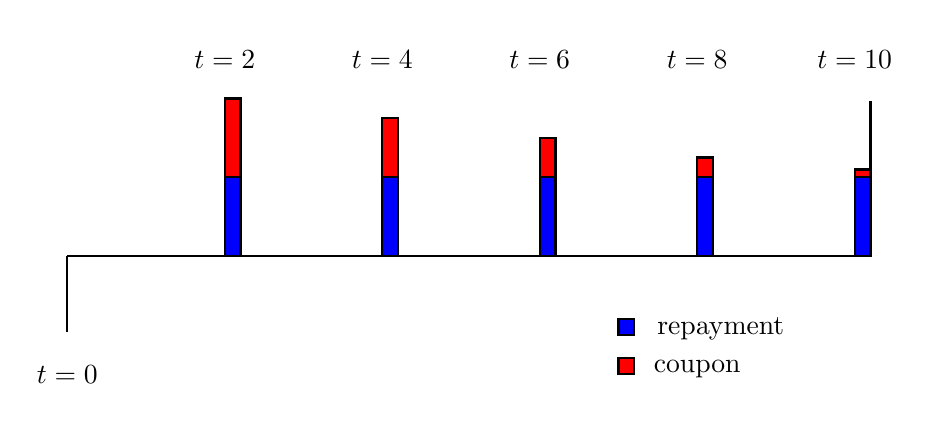
\begin{tikzpicture}[-,shorten >=1pt,auto,node distance=1.5cm,thick,minimum size=0.8cm,main node/.style={circle,draw=red,very thick}]
\tikzstyle{selected edge} = [draw,line width=6pt,-,blue!30]

\coordinate (belowstart) at (0,-1);
\coordinate (start) at (0,0);
\coordinate (stop) at (10.2,0);
\coordinate (abovestop) at (10.2,2);
\draw (start) -- (stop);
\draw (start) -- (belowstart);
\draw (stop) -- (abovestop);

\node at (0, -1.5) () {$t=0$};

\filldraw[draw=black, fill=blue] (2,0) rectangle node {} +(0.2,1);
\filldraw[draw=black, fill=red]  (2,1) rectangle node {} +(0.2,1);
\node at (2, 2.5) () {$t=2$};

\filldraw[draw=black, fill=blue] (4,0) rectangle node {} +(0.2,1);
\filldraw[draw=black, fill=red]  (4,1) rectangle node {} +(0.2,0.75);
\node at (4, 2.5) () {$t=4$};

\filldraw[draw=black, fill=blue] (6,0) rectangle node {} +(0.2,1);
\filldraw[draw=black, fill=red]  (6,1) rectangle node {} +(0.2,0.5);
\node at (6, 2.5) () {$t=6$};

\filldraw[draw=black, fill=blue] (8,0) rectangle node {} +(0.2,1);
\filldraw[draw=black, fill=red]  (8,1) rectangle node {} +(0.2,0.25);
\node at (8, 2.5) () {$t=8$};

\filldraw[draw=black, fill=blue] (10,0) rectangle node {} +(0.2,1);
\filldraw[draw=black, fill=red]  (10,1) rectangle node {} +(0.2,0.1);
\node at (10, 2.5) () {$t=10$};

% Legend
\filldraw[draw=black, fill=blue] (7,-1) rectangle node {} +(0.2,0.2);
\node at (8.3, -0.92) () {repayment};

\filldraw[draw=black, fill=red] (7,-1.5) rectangle node {} +(0.2,0.2);
\node at (8, -1.44) () {coupon};

\end{tikzpicture}
\caption{Cashflow of a serial.}
\label{fig:serialcf}
\end{center}
\end{figure}


\section{US Treasury Bonds}
Treasury securities are the debt financing instruments of the United States federal government, and they are often referred to simply as Treasuries.
\subsection{Treasury Bill - T-Bill}
Short term debt instruments that mature in one year or less.
\subsection{Treasury Note - T-Note}
Medium term debt instruments that mature in two to ten years.
\subsection{Treasury Bond - T-Bond}
Long term debt instruments that mature in twenty to thirty years.

\section{The term structure}
The term structure is defined as the zero coupon term structure.

\section{Term structure fitting methods}
Various methods of fitting a yield curve to data (LIBOR, forex futures, bonds).

\section{Interest rate swaps}